\chapter{Learning the evaluation function}
\label{chap:learning}
{\chapterintro
The previous two chapters described the facets of the playing agent.  In this chapter, the focus returns to the learning agent.  A review of the predominant learning methods is provided, and the learning framework is introduced.  This framework represents a key contribution of the current work, and the details of the framework is presented in the two chapters that follow this one.
}
\section{Introduction}
The playing performance of an agent is improved by increasing the search capabilities, or by strengthening the knowledge of the agent (see \refsec{knowledge-and-search}).  This chapter provides a review of the methods used to improve the game knowledge of the playing agent.  This learning task is the responsibility of the learning agent.    

As a starting point for learning, the zero-knowledge agent defined on page \pageref{def:zero} prescribes that learner should not be equipped with any game knowledge other than the knowledge contained in the game rules.  In order to argue that learning has occurred, Minsky \cite{minsky:steps} suggests as the minimum criterion that such an agent learns to play a better-than-chance game. 

The definition of the zero-knowledge agent does not place any constraints on the learning environment. Clearly, the environment in which the agent learns would have a marked influence on its learning performance.  In this environment, the agent could be provided with examples obtained from related literature, it could be guided by the interactive feedback of an expert, or it could learn on an on-line game server.  The latter training environment was used to train Baxter's \mygame{Chess} program, Knightcap \cite{baxter:chess} and in Fogel's Blondie \cite{fogel:edge}. It learned by playing on an Internet chess server against human players. On this server, human players tend to compete against opponents of their own strength.  Consequently, as Knightcap's strength increased, so did the strength of its opponents.  

The variety of environments and different objectives of the researchers (as highlighted in \refsec{motives}) lead to a large number of approaches to game learning.  The collection of techniques described in this chapter is not the result of a complete literature survey.  Methods considered to be  generally important and those that are directly related to the techniques developed for the current study are described.

The knowledge representation method described in Chapter \ref{chap:kr} encapsulates knowledge in a linear evaluation function. \refsec{learning-phased-function} discusses the problems introduced by this linearity and the use of game phases as a remedy to these problems. In \refsec{learning-features}, the challenge of feature discovery is discussed and the approach used by GLEM to identify features is reviewed.  This is followed by \refsec{learning-weights} that describes the application of machine learning techniques to the training of the evaluation function's weights.

An overview of the learning framework is provided by
\refsec{learning-framework}.  Specific attention is given to the macro-cycle of the framework. 
\refsec{learning-performance} describes a method that is used in subsequent chapters to compare the performance of playing agents. \refsec{learning-conclusion} concludes with a summary of this chapter. 
%
%The evaluation function that has to be approximated consists of features and weights (** ref to previous section **).  This chapter considers the problem of deciding which features to use in this function.
%
%\cite{minsky:steps}: Intelligence can be demonstrated by complex performances that we do not understand.  Because, we are programmers, we should not conclude that programs do not think - although the do what they are told, the consequences of the  actions taken by learning programs  is not known.
%
%\cite{kubat:review} A learning system must be able to deal with imperfections in the data.  Examples often contains a certain amount of noise.  Noise is errors in descriptions or errors in the classification.  Also, examples can be incomplete in the sense that some attribute values are missing.  
%
% construction vs. selection
%\cite{utgoff:feature} In principle it is possible to provide the agent with all possible features and it could decide which of these are `in' or 'out'.  This is a {\it feature selection} approach.  Alternatively, the agent can start with no features and construct any feature and delete features when it is no longer needed.  The latter is a {\it feature construction} approach.  
%  
% \cite{fawcett:systems} **Why can we not use primitive features? **examples vs. training instances ** overfitting (pool page 408) and underfitting  babosity ** connectionist learning ** induction learning  ** convergence
%
%\section{Features}
% how should the feature set be composed
%\cite{utgoff:feature}  The problem of defining good features becomes the problem of finding useful intrinsic properties of the domain elements.  Several issues influence the usefulness of the set of features to be used in the function:
%\begin{mydesclist}
%\item{Linear independance}.  When aiming for a function that minimises the mean-squared error in an approximation, linear independent features are less likely to become trapped at a local minimum.  Although a local minimum may produce a useful function, such situations are best avoided.  
%\item{Orthogonality}. The weights of orthogonal features can be adjusted independently of each other and consequently learning becomes faster.  Features that overlap are not orthogonal - and more overlapping features slows down learning.
%\item{Feature domain size}.  The weight of features with large domains will be adjusted more often than the weights of features with smaller domains.  This is because the weight is adjusted when the feature covers (i.e. is present on) the example domain element.  
%\item{Covering domain element sets}.  How does the feature split the domain: {\it axis-parallel} or {\it oblique}. **(need more clarity on these)  
%\end{mydesclist}
%
%\section{Existing approaches} 
%(**\cite{utgoff:feature} provides an in depth description of the problem of feature construction)
%\section{Zenith}     
%\cite{furnkranz:survey}
%**\cite{fawcett:systems} created the Zenith system which automatically constructs features represented as first-order predicate calculus.   New features can be derived by decomposition, regression and specialization of old features. 
%\section{Elf}
%\cite{furnkranz:survey}
%**\cite{utgoff:approximation} constructs new features as a set of basic, Boolean evaluation terms in Elf.  (TODO: summarize method from **\cite{utgoff:approximation})
%
% when does learning occur?
% \section{Introduction to learning concepts}
%
% meaning of induction
%\cite{poole:learning} An \myterm{induction algorithm}  takes as input specific instances and infers a model that generalizes beyond these instances. It can be contracted with {\it deduction} which is the derivation of the consequences of a knowledge base and {\it abduction} which is hypothesizing what may be true about a particular case.
% \cite{poole:learning} A \myterm{bias} is a tendency to prefer one hypothesis over another.  If hypothesis A and hypothesis B accurately predicts the data, something external to the data must be used to choose.  If an unseen data arises on which A and B does no agree, no decision can be made for this data without a bias.    Therefore a bias is needed for any inductive process that makes predictions on unseen data.  What constitutes a good bias is an empirical question about which biases work well in practice.  In choosing a hypothesis a common justification is to choose the simplest hypothesis - that is Ockham's razor.  According to Ockham: ''what can be done with fewer is done in vain with more".  This principle works because it is reasonable to assume that there is structure in the world to be discovered and it is efficient to explore the simplest hypothesis first.  

%meaning of generalisation
% \cite{kubat:review} Given a single labelled example of a concept, the learner knows the \myterm{most specific} description of the concept and nothing more.  Any generalisation is possible at this point.  Only after receiving negative examples, some constraints are imposed on the generalisation.  This produces a set of the \myterm{most general} descriptions - these cover the position but not the negative examples.  Further negative examples may reveal that this set is \myterm{overgeneralised}, resulting in a further specialisation of the set.  New positive examples provides another most specific description, which calls for another generalisation.   In other words, positive examples introduces generalisations and negative example may result in specialisations of descriptions.  Thus, the learning of a concepts can be seen as the search through a space of descriptions where the essential search operators are generalisation and specialisation.  Besides the choice of representation language, the proper selection of these search operators is the most critical task of the designer of a learning program.
%
%\section{Considerations}
% Search parameters
% \cite{kubat:review} If one views concept learning as a search through the generalisation space, each state in this search tree represents a description of the concept.  A commitment must be made to the \myterm{initial state} - typically this corresponds with the positive examples.  The \myterm{termination criterion} is the objective and states that satisfies this criterion are referred to as \myterm{final states}.  For example, the termination criterion can be that the description covers all positive and no negative examples.  The \myterm{search operators} that advances the search from one state to another are typically the generalisations and specialisations of the descriptions.  And finally, a \myterm{search strategy} the states to be explored and under what conditions an operator is to be applied.

\section{The phased evaluation function}
\label{sec:learning-phased-function}
A reason for choosing non-linear representations such as neural networks for game learning is that these techniques are able to  approximate a much larger class of evaluation functions than linear representations. Berliner \cite{berliner:beats} describes a problem with linear functions, called \myterm{suicide construction}. Consider a simple term in a linear function, $S = I \times D$, where $S$ denotes suffering, $I$  pain intensity and $D$ denotes pain duration.  If the aim is to minimise suffering, this term seems like reasonable advice: reduce $I$ and  $D$. If the program is able to manipulate the value of $D$, and an excruciating pain cannot be removed, it may well recommend suicide by driving $D$ to $0$.  This advice would usually not be a valid solution.  However, when this term appears amongst others in a linear evaluation function in which other terms place a high value on staying alive, the value of $D = 0$ might be taken.  In other words, suicide construction occurs when the potential exists for one of the weights to be adjusted in an undesirable direction.

Given a linear representation for the evaluation function, non-linearity can be introduced by separating the game into phases, and assigning a different evaluation function to each phase. The result is a composite function called a \myterm{phased evaluation function}.  Clearly, the possibility remains to use  neural networks instead of linear functions as the parts in this composition. Boyan \cite{boyan:masters-thesis} explored this possibility using \mygame{Backgammon} as domain. His results indicate that using a different network for each game phase is an improvement over learning the weights of a single neural network for the entire game. 

There are many ways to define the phases for a given game. Boyan identified 12 game phases for \mygame{Backgammon}, and trained 12 networks.  He determined the game phase from the pip count\footnote{The Pip Count is the total number of points that a player must move his pieces to bring them home and bear them off. At the start of a game each player has a pip count of 167.} for each player. The player's pip count for contact positions\footnote{A contact position is one in which one or more pieces of the players are (or can potentially be) on the same point position.}  is classified as small, average or large.  Pairing the pip count classification of the players gives rise to 9 game phases: \{(small,small),(small,average), \ldots , (large,large)\}.  The remaining 3 phases categorises the non-contact positions.  A non contact position can be in one of 3 states: (a) the first player leads, (b) the second player leads, or (c) the race is relatively close.  

The phases used by Lee and Mahajan \cite{lee:pattern} for  \mygame{Othello} is much simpler. They use the total number of discs on the board to determine the game phase.  Their learner focussed on the middle game and 26 (out of 64) phases were used during training: from the $24^{th}$ phase to the $49^{th}$ phase.  The training problem was to find the weights for four hand-coded features. The results obtained by Lee and Mahajan show an improvement in the performance of an \mygame{Othello} program that already played at world championship level.
%
%They smoothed training information by sharing training examples that were within two moves of the target phase. 
%
%A particular problem with the phased approach, called the \myterm{blemish effect} \cite{berliner:construction}, has to be addressed. "a very small change in the value of some feature could produce a substantial change in the value of the function. When the program has the ability to manipulate such a feature, it will frequently do so to its own detriment".

\section{Discovering features}
\label{sec:learning-features}
Nearly five decades before this writing, the challenge to automatically discover game features  was set by Arthur Samuel \cite{samuel:checkers}. Samuel's challenge implies the discovery of features that can be used in place of the hand-crafted features used by his linear evaluation function.  However, the non-linear, neural network approach proved to be an effective knowledge representation technique that is ideally suited for traning.  

As an evaluation function, a neural network encapsulates knowledge in three ways: the network topology, the weights and the encoding.  Encoding refers to the process that translates the game position into the floating-point values that are assigned to the input nodes of the network. The encoding is usually a fixed procedure, and conceptually node weights correspond with the weights in a linear function. It is possible to `discover' an optimal network topology. Consequently, one may expect the problem of identifying the topology of a neural network and the problem of finding features for a linear evaluation function to be related.  However, the two problems are very distinct, and little synergy can found in the methods used.  The main difference is that linear feature discovery expects to find highly structured information while an optimal neural network architecture represents an optimal structure for the non-linear function.  

The problem of finding a neural network architecture revolves around the structure of the hidden layers in the network. One approach is to have a single hidden layer and to determine the number of nodes in this layer.  This approach was used by Fogel for an  agent that learns how to play \mygame{Tic-tac-toe} \cite{fogel:networks}.  Moriarty and Miikulainen \cite{moriarty:evolving} takes on the more complicated problem of also determining the number of hidden layers in the architecture.  Their program uses \mygame{Othello} as learning domain.

The discovery of features for a linear evaluation function is closer to the aim of the current work.  In the subsection that follows, an approach developed by Michael Buro to learn such features is described in detail. He also used \mygame{Othello} for his learning experiments.

\subsection{GLEM configuration discovery}
\label{sec:learn:GLEM}
Micheal Buro introduced the Generalised Linear Evaluation Model (GLEM) to discover the terms of a linear evaluation function \cite{buro:feature}. The GLEM representation scheme and GLEM configurations have already been described in \refsec{knowledge-granularity}.  A GLEM configuration is a combination of GLEM atomic features, and can (in a more general sense) be regarded as a feature in a linear evaluation function.  Consequently, the approach used by GLEM to identify a set of configurations is essentially an approach to discover evaluation function features. 

The number of possible configurations for a set of GLEM atomic features $\{f_1,f_2,\ldots,f_k\}$ grows exponentially with the size of the set.  If all the atomic features are binary, there are $2^k$ possible configurations.  However, the possibilities are typically much more than $2^k$ because a GLEM atomic feature is likely to have more than two possible values, and a valid configuration does not need to contain all the atomic features.  Hence, it is impractical to enumerate all the possible configurations in an evaluation function and then to find optimal weights for them.  Also, most of these combinations that will not be useful in an evaluation function.  There are certain combinations describe positions that are impossible to attain: for example, having all 8 your pawns in the $7^{th}$ rank during a \mygame{Chess} game.

Buro's deduction process \cite{buro:feature} decides on a set of \myterm{active configurations} based on a large set of example positions, $E$, and a cut-off value $n$. The algorithm includes a configuration in the active set if and only if there are $n$ or more instances in $E$ that match the configuration. A higher value of $n$ reduces the risk of overfitting.  \refalg{glem_discovery} outlines the most basic implementation of this algorithm.
\begin{figure}[h!]
\begin{algorithm}
{GLEM Discovery}
{A set of examples $E$, a set of features $F$ and a cut-off value $n$.}
{A set of configurations $C$} 
GlemDiscover(E,F,n) \+\\
	Set $R$ to the most general values in $F$ \label{line:glem_general} \\
	$C = R$ \\
	$N = R$ \\
	while ($|N| > 0$) \+\\
		$M = \{\}$ \\
		for each $c_j$ in $N$ \+\\
			for each $r_k$ in $R$ \+ \\
				$e = c_j \myunion r_k$ \\
				if ($e$ is found no less than $n$ times in $E$) \+\\ 
					$M = M \myunion \{e\}$ \-\-\-\\
		$N = M$ \\
		$C = C \myunion N$ \-\\			
	Remove all general configurations from $C$	\label{line:glem_specific} \\
	return $C$ 
\end{algorithm}
\caption{An outline of the GLEM discovery algorithm}
\label{alg:glem_discovery}	
\end{figure}

In \refline{glem_general} of the outline, the set $C$ is initialised to the set of most general elements, $R$. An element in this set is a feature combined with an element from the feature's domain.  For example, an atomic feature called {\it color} with domain {\it \{red,green,blue\}} would contribute 3 most general elements to the set.  $R$ is also used in the inner loop of the algorithm.  Here, every configuration in $N$ (initially set to $R$) is combined with an element in $R$ and if the new combination is supported by more than $n$ examples, it eventually becomes an element in $C$.  This process is repeated with all the new elements identified in the {\tt while} loop until no new configurations are found.  

A combination $a$ is more specific than a combination $b$ if an only if $a$ contains all the elements in $b$ and $a$ has more elements than $b$.  For every combination in $C$, created during the collection cycle that has a length greater than one, the same combination with the last atomic feature removed is also in $C$.  Thus, most of the combinations collected are generalisations of other combinations that are also collected.  The final step of the procedure (\refline{glem_specific}) returns $C$ after all the general configurations are removed from this set.

Buro's contribution \cite{buro:feature} includes novel techniques to improve the computational efficiency of the algorithm itself and also the efficiency of the access to, and the storage of the resulting data structure. 

Essentially GLEM expressions are two levels deep - the first level contains the configuration, and the second contains the atomic features.  The feature language, $\mathcal{F}$, introduced in \refsec{knowledge-language} is a much richer representation method, that allows complex expressions of arbitrary length.  In addition, the atomic features used in $\mathcal{F}$ are less coarse than GLEM's atomic features.  These two differences make the number of possible expressions in $\mathcal{F}$ much more that the possibilities in GLEM.  It is therefore not practical to use GLEM to find $\mathcal{F}$ expressions from a set of example positions.    
%** Comments -- discovery process does not use labelled examples -- the process does not attempt to identify "better" and "worse strategies"   
%
%GLEM and the concept of a GLEM configuration is described in . 
%\cite{furnkranz:survey}
%GLEM uses an efficient algorithm that is quite similar to the well known Apriory data mining algorithm **\cite{agrawal:fast}.   Contrary to Elf,where  both weights and features are updated online and simultaneously, features in GLEM are constructed in batch and weights are determined in a second pass by linear regression.   
%The \textit{building block approach to genetic programming (BGP)} is based on a few assumptions: 
% \begin{itemize}
% \item The \textsl{complete data assumption} states that the training examples
%must not contain omissions or unknown elements.  This fits the concept of
%perfect-information games like a glove:  Positions do not have omissions on
%unknown elements. 
%\item The \textsl{complete classification assumption} states that each instance
%maps to one and only one classification.  A described above, each training
%example has exactly one classification chosen out of a possible eight.     
%\item The \textsl{limited data types assumption} states that attributes must be
%discreet or continuous numbers, unordered nominal or Boolean.  For the
%evaluation function, all attributes are Boolean.  It is possible that this
%simplification makes BGP more suitable for the evaluation function problem than it was for its original application to data mining. In that application, BGP did show a weakness when dealing with many continuous attributes.
%\end{itemize}
% 
% Many of the detail to make BGP work is omitted from this paper, such as the selection of crossover and mutation operators.  It is unlikely that any change in this regard would be made to the original BGP.  However, richer semantics can be expected to prevent the generation of irrational nodes, and also to minimise the occurrence of equivalent nodes in the population.

\section{Learning weights}
\label{sec:learning-weights}
The automatic optimisation of the weights of an evaluation function is the most extensively studied learning problem in game playing \cite{furnkranz:survey}. Like the feature discovery problem, the problem of finding optimal weights for game playing agents has also been more visible in the neural network arena.  In contrast to the feature discovery problem, the problem of finding optimal weights for a linear function and for a neural network that plays a game are very alike.  In both problems, the aim is to find a solution in a multi-dimensional space of floating-point values.  In addition, the problems share the same input (albeit encoded differently), and learns the same activity.  A variety of different approaches to solve this problem has been proposed. 

% examples 
Samuel \cite{samuel:checkers} provides his \mygame{Checkers} learning agent with a linear evaluation function composed from hand-crafted terms based on \mygame{Checkers} literature.  The sign of the weights was also part of the input.  Samuel remarks that the program could already play a `fairly interesting game', even before learning started.  

Pollack \etal \cite{pollack:player} trains a fixed neural network to play \mygame{Backgammon}.  The network's input nodes encode only visible features and a flag that indicates whether the game is in the endgame phase. 

Kotnik and Kalita \cite{kotnik:significance} trains the weights of a fixed neural network to play \mygame{Gin Rummy}.  In this case, the network does not encode visible features of the game state. The input nodes accept an encoding of the accessibility of the playing cards.  More accessible cards have a higher value, {\it i.e.} a card that can potentially be accessed by the player has more value than a card known to be in an opponent's hand.   

Franken and Engelbrecht \cite{franken:checkers} developed a \mygame{Checkers} learning agent that finds optimal weights for a neural network.  As input, this network takes a value for each square, such that a higher value indicates the contribution the square makes to the strength of the active player.  For instance, a square occupied by an opponent king has less value than an empty square or one that is occupied by the active player's king.  
 
Another recent example is the neural networks trained by Fogel \etal \cite{fogel:chess} for a \mygame{Chess} player.  In addition to the trained neural networks, the player was also equipped with an advanced tree search that extends when a position at the edge of the search meets certain criteria, as well as opening- and closing books.  The research problem addressed here is  to improve the skill of a very strong player.  In this case the input nodes accepted the material value of the piece on the square of the \mygame{Chess} board.

Although the specific learning problems and the representations are diverse, a relatively small number of different learning methods are employed by most of the researchers.  These methods are general approaches to the class of learning problems associated with weight training for games.  In the subsections that follow, supervised- and reinforcement learning are described as fundamental learning methods.  Temporal difference learning is a method that has been devised specifically for game learning.  In the last subsection, strategies to use coevolution as a game learning method are explored.

%\cite{furnkranz:survey}
%
%Known approaches to solve this problem of weight be categorised by the type of information they receive **\cite{furnkranz:survey}:
%\begin{mydesclist}
%\item In \myterm{supervised learning} each training instance is a game state labelled with the correct value for the evaluation function.
%\item In \myterm{comparison training} the training instances indicate preferences.  For example, the instances could be a pair of moves and an indication of which is preferable. Alternatively the training instance could be a collection of moves together with an indication of which moves were played.
%\item In \myterm{reinforcement learning} there are no training instances information about the absolute or the relative value of the positions or the moves. Instead, the program receives feedback from the environment on whether moves was good or bad.  In the simplest case, this feedback is the outcome of the game.  A special case of reinforcement learning is \myterm{temporal difference learning} in which the evaluation function values of later positions are used to reinforce correct decisions earlier in the game.
%\end{mydesclist}  

\subsection{Supervised learning}   
The \myterm{supervised learning} process typically uses a large collection of rated example game positions as input. The rating of an example is an expert's estimate of the value the evaluation function should assign to the position \cite{furnkranz:survey}. Successful training produces weights for the evaluation function such that the function correctly predicts the value of new  positions encountered during play. Essentially, the evaluation function generalises the specific information supplied in the form of rated examples.  

The challenge of supervised learning is to acquire accurate ratings for examples. The value assigned by an expert to a particular example is a subjective value; and there is no absolute standard to measure the correctness of his assessment.  Incorrectly rated examples complicate the generalisation process and lead to ineffective training. Consistency is more important than absolute accuracy. As long as the ratings provide the learner with enough information to decide the direction in which to adjust the weights, the examples are adequate. 

The success of the achievements of Tesauro has to be partly due  to the knowledge he has of \mygame{Backgammon}. As an expert player, Tesauro himself provided the ratings for the initial work he conducted on this game \cite{furnkranz:survey,tesauro:network}. However, for the typical research endeavour, experts are not readily available and the rating process is a time-intensive and costly ordeal \cite{furnkranz:survey}.

A common method used for supervised training adjusts the weights such that the mean squared error is minimised.  This error measure is calculated as follows for a set of weights, $\vec{x}$:
\[
E(\vec{x}) = \frac{\sum_{i=1}^{N} (F(\vec{x},e_i) - R(e_i))^2}{N}
\]
where $F(\vec{x},e_i)$ is the evaluation function value for example $e_i$, and $R(e_i)$ is the rating for example $e_i$.  
This equation was used by Buro \cite{buro:statistical, buro:feature} and Mitchell \cite{mitchell:masters} to train \mygame{Othello} players.  

\myterm{Comparison training} is an approach introduced by Tesauro \cite{tesauro:comparison} that does not use quantitative ratings.    Instead of rating each individual example separately, the expert is given a set of examples, and he decides which of the examples in the set is the best, and which example is the worst.  The training objective for comparison training is to maximise the number of correct choices made by the evaluation function when it is presented with the same example sets.

If the research aim is to train a playing agent that is able to beat top human players, supervised learning is not a practical option.  Even if enough correctly rated (or compared) examples are available, the learner still generalises over the examples. As a generalisation, the learner may achieve very high levels of playing performance, but it will not discover a novel strategy that will surprise an expert player.  In effect, such a learner will be unable to beat the expert(s) that provided the ratings for the examples from which it obtained the generalisation.     
%
%
%In contrast to the findings by Lee and Mahajan **\cite{lee:pattern}, Buro **\cite{buro:statistical} concludes that the presence of feature correlations is not a sufficient condition to use a non-linear function, he argues that it only pays off if the covariance matrices are different.   
%
%\subsection{Supervised learning}
%\cite{furnkranz:survey}
%During function tuning, the weights must be adjusted such that the error of the evaluation function value on the training instances are minimised. The resulting function can be learning by linear optimisation or a non-linear optimisation technique like back-propagation training for neural networks. Buro also used error minimising.
%Mitchell  applied a linear method to tune an evaluation function for the game of \mygame{Othello}.  The function consisted of 28 weighted features. He selected 180 example positions that occurred in tournament play after the 44th move and determined the game theoretic value of each of these positions with an exhaustive search.  
% Another Othello program developed by Lee and Mahajan \cite{lee:pattern} obtained training instances by playing against itself.  In order to obtain a variety of games, the first 20 moves were made randomly.  Each training position was labelled with won or lost and the value of four different numeric feature scores.  Using statistical methods, optimal weights for hand-crafted features were determined.  Buro \cite{buro:statistical} used a similar approach.
%\subsection{Comparison training}
%\cite{furnkranz:survey}
%In Tesauro's framework  constraints are placed on the network architecture  to ensure that the network remains consistent.  For comparison training, a consistent choice is both transitive\footnote{if $a < b$ and $b < c$ then $a < c$} and symmetric\footnote{if $a < b$ holds then $b < a$ does not hold}.   
\subsection{Reinforcement learning}
%\cite{furnkranz:survey}
\myterm{Reinforcement learning} \cite{sutton:learning} is a learning process whereby an agent learns which action to take from feedback information it receives from the environment.  This information, called \myterm{reward}, is received after the learner takes one or more actions. If the reward for an action is positive, the action is reinforced, and the tendency of the learner to take that action again in the future is increased. A negative reward decreases the tendency to repeat the action that was taken.  

The \myterm{learning rate}, $\theta$, is a positive floating-point parameter to the reinforcement learning process ($\theta < 1$).   This parameter controls the rate at which the agent adjusts its behaviour based on each reward.  A high value for  $\theta$ increases the learning rate and the agent adapts quicker when a reward is received. A low value slows down the learning progress, but it is more reliable in the uncertainty caused by the noise that is typically present in the feedback process.     

% example adapted from \cite{minsky:steps}
As an example, consider an agent that must choose between two actions: turn left or turn right. The learning exercise is to teach the agent that it must always turn right. Internally, the agent keeps a probability value by which it chooses to turn right.  The initial value for this probability is $0.5$. Let the sequence $p_1,p_2,  p_3,\ldots $ represent this internal probability value as it changes over time ($p_t$ is the probability before the $t^{th}$ action is taken). At time $i$, the agent turns right and it receives a positive reward. In this case $p_i$ is adjusted as follows:
\[ p_i = p_{i-1} \times (1-\theta) + \theta \]
Conversely, if the agent turns left it receives a negative reward and $p_i$ is adjusted as follows:
\[ p_i = p_{i-1} \times (1-\theta) - \theta \]
This example clearly demonstrates the role of the learning rate.  A low rate elevates the importance of the experience gained thus far, whereas a high value for $\theta$ considers the last feedback as more important. After a number of attempts, the probability by which the agent chooses to turn right will increase and eventually the agent will always turn right. 

%\cite{furnkranz:survey}
The term \myterm{delayed reinforcement} is used to describe a reinforcement learning process where more than one action is taken before a reward is received. The delayed feedback is typical of the games of interest to the current study; only after an entire sequence of moves are made, the outcome of the game becomes available. The actions available to the game learning agent are presented as the list of available moves at each decision point in the game. Typically, the actions are reinforced or penalised by increasing or decreasing a score associated to the position on the play-line. The score adjustment for a draw is somewhere between the positive adjustment for a winning position and the negative adjustment for a losing position.  

It is possible that a lost game is caused by one bad move, and the other moves in that game are good moves.  In such a case, only the culprit move should receive a negative reward. Unfortunately, the learning agent is usually unable to distinguish the bad moves from the good moves in the play-line.  This leads to the \myterm{credit assignment problem} \cite{minsky:steps}. This problem concerns the method by which the reward is distributed to the individual actions responsible for it. Two simple approaches are practical \cite{michie:game}: the first is to distribute the reward equally amongst all the moves that contributed, and the second option is to increase the proportional assignment for positions that occur later in the game.  This proportional assignment is based on the premise that initial moves have a lesser impact on the outcome of the game than moves in the endgame.  Clearly, these approaches do not solve the assignment problem for a specific game line. However, after applying a consistent approach over a multitude of training games, the score of a position becomes more accurate.

During the initial training of reinforcement learning it is possible that some properties are mistakenly chosen to be important.  The problem of ``unlearning" this knowledge can hinder learning progress at a later stage \cite{minsky:steps}.  This problem can be mitigated by choosing the training sequences well.

The basic process of reinforcement learning is problematic for non-trivial games. In these games, the likelihood of coming across the same middle game position is very low. During play many positions are encountered that have not yet been scored.  For these games some kind of generalisation over positions is required.  One method is to assign the reward to a class of positions, and not to an instance. A related problem is that training on the outcome of games is a slow process because many games are needed before the scores converge to accurate values \cite{buro:statistical}.
%Sutton and Barto  convergence theorems regarding the convergence of reinforcement learning has been proven **\cite{sutton:learning}.
%F\"urnkranz \cite{furnkranz:survey} suggests that the distinction between reinforcement and supervised learning becomes unclear when the evaluation function is tuned during play using feedback received after each move.  This scenario is possible in certain games (like the card game \mygame{Hearts}). The reason for this is that each move can be regarded as an accurately rated training instance.
%% ** some more clarification of what furnkranz meant here is needed
\subsection{Temporal Difference learning}
%\cite{sutton:temporal}
Temporal difference learning (TD) is a reinforcement learning process that mitigates the problems associated with delayed reinforcement.  When the reward is immediate, the behaviour of TD is no different than the reinforcement learning process described in the previous section.  However, when a \myterm{multi-step activity} is learnt, TD converges faster and produces better predictions than the basic reinforcement approach \cite{sutton:temporal}.  

The key to understanding TD is to consider the sequence of observations, $\vec{x}_1, \vec{x}_2, \vec{x}_3, \ldots, \vec{x}_m$ that leads to the outcome $z$.  Each vector $\vec{x}_t$ describes the state of the environment at time $t$; and $z$ is the outcome at time $m$. The aim of the TD learner is to produce a corresponding sequence of predictions of the outcome ($z$), say $P_1,P_2, P_3, \ldots, P_m$.  At time $t$, the prediction for $z$ is $P_t$.  If these predictions are accurate, the player is able to determine at time $t$ which move would lead to a winning outcome because the prediction, $P_{t+1}$ for the resulting position, $\vec{x}_{t+1}$  will be a win.

Each prediction is based on a vector of modifiable weights, $\vec{w}$. Thus, $P_t$ can be denoted as $P(\vec{x}_t,\vec{w})$.  During learning, the values of $\vec{w}$ is updated.  

Consider an approach to determine the value of $\vec{w}$ after  the sequence (of $m$ steps) is complete and the outcome is known to be $z$.  The supervised learning process would use the position-outcome pairs $(\vec{x}_1,z),(\vec{x}_2,z),(\vec{x}_3,z),\ldots,(\vec{x}_m,z)$ as rated examples.  An assignment can be made to $\vec{w}$ that satisfies the equation $P(\vec{x}_m,\vec{w}) = z$.  Now, for each observation leading to $\vec{x}_m$ an increment as $\Delta\vec{w}$, is determined and $\vec{w}$ is the sum of these increments:
\begin{equation}
\label{eq:delta_sum}
\vec{w} = \sum_{t=1}^{m} \Delta \vec{w}_t
\end{equation}
The increment, $\Delta \vec{w}_t$, depends on the difference between $P_t$ and $z$, and how a change in $\vec{w}$ will affect the value of $P_t$.  For supervised learning a learning rate, $\theta$ and a gradient, $\nabla_{\vec{w}} P_t$ can be used to determine the increment:
\begin{equation}
\label{eq:delta}
\Delta \vec{w}_t = \theta(z - P_t) \nabla_{\vec{w}} P_t
\end{equation}
The gradient, $\nabla_{\vec{w}} P_t$ is the vector of partial derivatives of $P_t$ with respect to each component of $\vec{w}$.  For the special case where a linear function, $P_t$ is learnt: 
\begin{equation}
\label{eq:linear}
	P_t = \vec{w}^T \vec{x}_t = \sum_{i} \vec{w}(i) \vec{x}_t(i)
\end{equation}
where 	$\vec{w}(i)$ and $\vec{x}_t(i)$ are the $i$-th components of  $\vec{w}$ and $\vec{x}_t$ respectively.   In this case,$\nabla_{\vec{w}} P_t = \vec{x}_t$ (it is  the derivative of  \refeq{linear} with respect to $\vec{w}$), and  \refeq{delta} is reduced to the Widrow-Hoff rule \cite{widrow:circuits}:
\begin{equation}
\label{eq:widrow}
\Delta \vec{w}_t = \theta(z - \vec{w}^T\vec{x}_t) \vec{x}_t
\end{equation}   

The difference $z - \vec{w}^T\vec{x}_t$ represents the scalar error between the prediction and what it should have been.  This error is multiplied by the vector $\vec{x}_t$ because $\vec{x}_t$ indicates how each weight must be adjusted to reduce the error.  For example, if the error is positive, $\vec{x}_t[i]$\footnote{$\vec{a}[b]$ refers to the $b^{th}$ element of $\vec{a}$} is positive and $\vec{w}[i]$ will be increased - resulting in an increase of $\vec{w}^T\vec{x}_t$ and reducing the error.

The equation to determine $P_t$ is dependant on $z$, and $P_t$ cannot be computed before $z$ is known.  In other words,  \refeq{widrow} cannot be calculated incrementally.  There is a temporal difference learning procedure, called TD(1) that produces the same result as  \refeq{widrow} such that the value can be computed incrementally.  Let $P_{m+1}  \equiv z$, then the error at $P_t$ is the sum of the changes in the predictions after $P_t$:
\[
	z - P_t = \sum_{k=t}^{m}(P_{k+1} - P_k)
\]  
From  \refeq{delta_sum}, the linear weights are determined as follows:
\begin{eqnarray}
\nonumber \vec{w} & = & \vec{w} + \sum_{t=1}^{m}\theta(z - P_t) \vec{x}_t   \\
\nonumber & = & \vec{w} + \theta \sum_{t=1}^{m} \sum_{k=t}^{m}(P_{k+1} - P_k) \vec{x}_t 
\end{eqnarray}
Because $\sum_{i=1}^n\sum_{j=i}^n a_ib_j = \sum_{j=1}^n\sum_{i=1}^j a_ib_j$:
\begin{eqnarray}
\nonumber \vec{w} & = & \vec{w} +  \theta \sum_{k=1}^{m}\sum_{t=1}^{k}(P_{k+1} - P_k) \vec{x}_t \\
\nonumber & = & \vec{w} + \sum_{t=1}^{m}\theta(P_{t+1} - P_t) \sum_{k=1}^{t} \vec{x}_k 
\end{eqnarray}
The increment can now be expressed as: 
\begin{equation}
\label{td_delta}
\Delta \vec{w}_t = \theta(P_{t+1} - P_t) \sum_{k=1}^{t} \vec{x}_k
\end{equation}

The value of $\Delta \vec{w}_t$ can be computed incrementally  because it depends on the value of the two successive predictions and the sum of all preceding increments.   In response to a new prediction, $P_{t+1}$, $\Delta \vec{w}_t$ can be determined and used to update the predictions, $P_1, P_2, \ldots,P_t$.  The TD(1) procedure alters all these to an equal extent.  TD($\lambda$) is a class of procedures that make greater alterations to more recent predictions: the prediction for an observation $k$ steps in the past are weighted by $\lambda^k$ where $\lambda \in [0,1]$:
\begin{equation}
\label{eq:dwt}
\Delta \vec{w}_t = \theta(P_{t+1} - P_t) \sum_{k=1}^{t} \lambda^{t-k} \vec{x}_k
\end{equation}
A larger value for $\lambda$ increases the number of preceding observations that has an influence on the value of $\Delta \vec{w}_t$.  For TD(1), all the preceding observations are considered, and for TD(0) none of the preceding observations have an influence on the weight increment. 

The advantage of using the exponential form to alter the weights is that it can be computed incrementally: that is, the value $\Delta \vec{w}_{t+1} $ can be computed using the values obtained from the computation of $\Delta \vec{w}_t $.  The way this is done is shown in the following derivation:
\begin{eqnarray}
\nonumber \Delta \vec{w}_{t+1} 
	&=
	& \theta(P_{t+2} - P_{t-1}) 
	\sum_{k=1}^{t+1} \lambda^{t+1-k} \vec{x}_k \\
\nonumber 
	&= 
	&\theta(P_{t+2} - P_{t-1}) (\vec{x}_{t+1} + 
	\underbrace{\sum_{k=1}^t \lambda^{t-k} \vec{x}_k} _{\mbox{\tiny from  \refeq{dwt} }}) 
\end{eqnarray}

In order to gain an intuitive understanding of how TD learning works, consider a particular game position $q$.  From experience, the probability of winning from $q$ is estimated at $0.10$.  In a particular game line that leads to a win, another position, $p$, precedes position $q$. What is the estimated probability of winning associated to $p$?  Assuming $p$ was encountered only once during training and it lead to a win, a supervised learning method would conclude that $p$ is a good move.  The TD method would use $q$'s estimate to determine $p$'s value because $q$ precedes $p$.  The low estimate of $0.10$ for $q$ would lead TD to the conclusion that $p$ is more likely to lead to a loss.  If $q$ is correctly rated, the TD method is more correct.  Given infinite experience, both methods would converge to the same value for $p$, but when the  experience is limited, TD learns a better evaluation.  

Samuel's \cite{samuel:checkers} \mygame{Checkers} learner also adjusts the weights in accordance with the immediate successors in a game line.  The difference is that Samuel's program does not utilise an \textit{a priori} rating of the positions, while TD requires that every training sequence ends with a definite, externally supplied outcome. Samuel's decision to fix the weight of the most prominent feature (piece advantage), prevents his training procedure from finding useless evaluation functions. 
%
%This constraint discourages the procedure from finding useless evaluation functions.   The decision to set the weight with the largest absolute value to zero also could have prevented the program from exploring functions that has little to do with winning the game.  A simpler procedure than Samuel's explored by Christensen **\cite{christensen:static} obtained promising preliminary results.  
%Used by \cite{kotnik:significance}.

%\cite{furnkranz:survey}
Tesauro \cite{tesauro:practical,tesauro:learning} presented the first results of temporal difference learning on the training of an evaluation function for \mygame{Backgammon}. The trained playing agent, named TD-Gammon, achieved expert level play.
Other research attempts failed to achieve this level of performance, and TD's success has been attributed to the characteristics peculiar to \mygame{Backgammon} that makes it an ideal game for learning from self-play \cite{furnkranz:survey,pollack:player,kotnik:significance}. The primary characteristics cited is that the game does not require a large amount of search and that the dice-rolls guarantee the exploration of a sufficient variety of positions to identify all regions of the feature space.  

\subsection{Coevolution} 
\label{sec:learning-coevolution}
In the context of game learning coevolution is a learning process that involves adaptation of the environment in which the learner finds itself.  As the environment changes, the learner must adapt.  Coevolution also requires that the changes in the environment are largely a consequence of the changes in the learning agents. 

The simplest example of coevolution is two agents that learn by competing against each other.  In this case, one agent is the learning environment of the other. After each competition, the evaluation function of at least one of the agents are adjusted. This approach has been used by Pollack {\it et. el.} \cite{pollack:player} and Kotnik \cite{kotnik:significance} to train \mygame{Backgammon} and \mygame{Gin Rummy} players, respectively.  They compared their results with the TD approach and concluded coevolution works better than TD.  

This simple coevolution approach works well for \mygame{Backgammon} and \mygame{Gin Rummy} because these games are stochastic. The stochastic element ensures that a variety of match conditions are tested, even if the strategies of the competitors remain unchanged.  Thus, the accuracy of the assessment of stochastic competitors can be improved by increasing the number of matches played during a competition.  

For perfect information games, this simple strategy would not be effective.  In perfect information games, the outcome of the game is always the same when two players compete.  A win against a single opponent does not imply the winning player's strategy is better in general.  For this reason, coevolution learning for perfect information games typically involves a population of learning agents. 

Two approaches toward the coevolution of a population are popular.  The first is the use of a \myterm{genetic algorithm} (GA) in which the population evolves using natural selection and mutation.  The second approach is called \myterm{particle swarm optimisation} (PSO), where the population is modelled as a swarm that finds solutions by exploring the multi-dimensional problem space.  These approaches have a common challenge: the separation of the better individuals in the population from those individuals that do not perform well.  The strategy to rate the individuals in the swarm is encapsulated in a function called the \myterm{fitness function}.  

The use of a GA or a PSO does not always imply coevolution. Coevolution is not present when the environment used to rate  individuals is entirely static.  For instance,  the fitness function of a GA used by Tunstall-Pedoe \cite{tunstall-pedoe:genetic} uses a set of example moves.  The fitness of an individual depends on the number of moves chosen correctly when presented with these examples.  The training environment consists of a static example set, and thus Tunstall-Pedoe does not employ coevolution. Another example is the \mygame{Othello} learning agent of Moriarty and Miikulainen \cite{moriarty:evolving}. It initially plays against random moving players, and later against an advanced alpha-beta agent to determine the fitness of an individual.       

A simple mechanism to introduce coevolution into the fitness function is to measure the fitness of an individual using the other individuals in the population.  In game learning this mechanism is readily available due to the competitive nature of the activity that is learnt. This approach has been used to train a \mygame{Tic-tac-toe} player by Fogel \cite{fogel:networks},  Franken and Engelbrecht \cite{franken:evolving} and Messerschmidt and Engelbrecht \cite{messerschmidt:learning}. The same approach was also applied to the more difficult games, \mygame{Checkers} \cite{franken:checkers,chellapilla:without,fogel:edge}  and \mygame{Chess} \cite{fogel:chess}.  In these endeavours, the training involved the finding of optimal weights for neural networks. Davis and Kendall \cite{davis:evolve} used coevolution to find weights for a hand-crafted linear evaluation function that is used to play a perfect-information game called \mygame{Awari}.

In the GA approach, the population evolves in cycles called generations.  The fitness function determines the probability that an individual will become a parent of the new generation.  A new generation of individuals are built from the previous generation using the information of their parents.  A \myterm{cross-over} operator determines how the information from the parents are combined to form the individual for the new generation.  At a given probability, called the \myterm{mutation rate},  a \myterm{mutation} operator is applied to the offspring.  The purpose of this operator is to introduce new material into the population.

Fogel's \mygame{Tic-tac-toe} learner \cite{fogel:networks} avoids the cross-over operator by using a single parent.  He uses a mutation operator that makes random adjustments to the weights and adjusts the number of nodes in the hidden layer of the neural network. The \mygame{Chess} learner of Fogel \etal \cite{fogel:chess} also used a single parent and weight adjustment for mutation. Davis and Kendall \cite{davis:evolve} used the same approach for their GA.   

The PSO algorithm uses the fitness function to identify individuals in the population to which other individuals are attracted.  Using the same fitness function, PSO has been shown to be an improvement on GA \cite{franken:checkers,franken:evolving,messerschmidt:learning}.  For this reason, PSO is selected as the method to be used by the current research.  The detail of the PSO algorithm and how it is used in the game learning domain is discussed in a later chapter.
%The value domain of the weights  [-1;+1] interval; where a negative value    Searhc depth of 7.  
 %wduminy
%Although the results were in favour of  the simpler approach, Kotnik's experiment had a side effect that could provide an alternative explanation for his results.  The TD agent's reward is based on  the score ([0,1]), while the simple agent's reward is either 1 or 0.   The effect is that the training signal for a win (no matter how small the   winning margin) is much stronger (more discrete) for the simple agent  than it is for the TD agent.  Effectively the TD agent learns ``how to   win by a large margin" and the other agents agent learns ``how to win".  This is an unfortunate design decision that renders Kotnik's results inconclusive\footnote{May be a good idea for a small research project or a paper to do another comparison based on the same ideas proposed by Kotnik}.
% genetic algorithm
%\cite{messerschmidt:learning}, and therefore it is more difficult to learn as the second player. The network provided a score for each square. 
%\cite{fogel:networks} use score composed from competition against randomly chosen individuals from the population + against near-perfect player.  Only winners become parents.
%Fogel decide to learn the first player.  In \mygame{Tic-tac-toe}, the players are not equal, and the second player has the disadvantage \cite{messerschmidt:learning}, and therefore it is more difficult to learn as the second player. The network provided a score for each square.
%\cite{fogel:chess} uses 10 games (5 as white and 5 as black) against randomly selected opponents.
%\cite{davis:evolve} plays against all other elements in the swarm; one game at each side.  3 poinst for a win, 1 for a draw and 0 for a loss.
%\cite{kubat:review} provides a nice intro to genetic algorithms -- page 61
%\cite{pollack:player} 
%A learning method makes use of coevolution if it satisfies two requirements: 1) the objective is not to learn an absolute optimum, but one that is better within a competitive (or cooperative) context; and 2) a form of exchange between the properties of individuals from the competing (or cooperating) populations is present.  
%In .  During the learning process, the losing species adapts until it becomes the new winning species.   Pollack, Blair and Land \cite{pollack:player}  and  Kotnik  \cite{kotnik:significance} employs a very simple form of this type of coevolution in which  two populations of learning agents compete.  One population consists of a single individual - the \textsl{champion}.  A random exploration surrounding the weights of the champion makes up the individuals of the competing population.  If an agent from the second population beats the champion convincingly, the weights of the champion is adjusted (slightly) in the direction of the winning challenger.  
%In addition to the reference agent becoming harder to beat, Pollack \textit{et al} also changes the competition during the evolutionary process.  In order to beat the reference agent, the challenger initially had to win 3 out of 4 games.  After 10 000 generations, it needed to win 5 out of 6, and then after 70 000 generations  7 out of 8 games must be won.  This complication was introduced because of evidence that the likelihood of finding a better player increased as the reference agent's ability improved.  The result of their work was a backgammon player that could beat a strong computer player  called PUBEVAL  40\% of the games played. 
%(*** provide a comparitive overview -- with specific mention to PSO's use in game learning --- refer to the chapter on PSO ***)
%see **\cite{kennedy:swarm} for the initial comparison to PSO.
%*** \cite{messerchmidt:learning} plays better Tic-tac-toe than \cite{fogel:edge}.
%\section{Considerations}
%\subsection{Using phases to achieve non-linearity}
%\cite{furnkranz:survey}
%The use of linear combination of features to characterise game positions is an obvious choice when performance is important.  However, two factors hinder the tuning of linear evaluation functions: term dependence and program dependence.  Changes to the weight of one term may affect the correctness of weight settings in other terms.  Once tuned, the weights are optimised to work in a particular setting. For instance a different search depth or an alternative quiescence algorithm may alter the importance of the ability to recognise certain tactical patterns and render the optimised function useless.  
%\subsection{Strategies to select opponents}
%\cite{furnkranz:survey}
%The training strategy must provide the learner with information that is focussed enough to guarantee convergence towards a good evaluation function, but the information should also provide the variation required to allow the learning of a function that is generally applicable.  The problem of variety is especially important when learning from self-play.  In reinforcement learning, this problem is known as the trade-off between exploration of new knowledge and the exploitation of already acquired knowledge. 
%TD-Gammon did not have the problem because the dice-roll provided sufficient variety.  Although Tesauro does not fully agree with Pollack and Blair, claims this is the only reason why TD-Gammon performed so well **\cite{pollack:strategy}.   They back up their claims by using a simple hill-climbing strategy to train the weights of the network.  The fact that such a simple strategy works all is in itself quite remarkable.  
%
%Epstein **\cite{epstein:ideal} presents evidence that self-training does not perform well for deterministic games.  She developed a game learning system called Hoyle that learned during self play.  Optimal results were not achieved from self-play, perfect opponents or random players - and she demonstrated that a lesson-and-practice training strategy is superior.  In this strategy phases of training with an expert player are interwoven with phases of self-play. Hoyle relies on an hierarchy of advisors that vote for, or against a particular move.  The advisors are hand-coded, but game independent.  
%Two of these advisors, Patsy and Zone Ranger use knowledge that are based on visual perception **\cite{epstein:expertly}.
%Samuel's \cite{samuel:checkers} learning strategy also reduced the change of getting stuck on a local optimum.  In his procedure the weights are trained against a frozen copy.  When considerable progress was made, the current weights are transferred to the frozen copy and the procedure continues.  However, when no progress was detected, the function was changed radically by setting the largest (i.e. most significant) weight to zero. A similar approach was used by Lynch **\cite{lynch:draughts}.
%The exploration of different regions of the search can be ensured by learning from games in which some moves are made randomly **\cite{lee:pattern,fogel:networks,schraudolph:temporal}.  Angeline and Pollack **\cite{angeline:evolve} evolved Tic-tac-toe players in parallel with a genetic algorithm.  The fitness of the players was determined by having them play in a tournament.  
%An intuitively good procedure  is to learn by playing against a wide variety of opponents of all playing strengths.  The success of the chess program KnightCap was party due to the fact that it learned by playing on an Internet chess server.  As human players tend to match with opponents of their own strength, the strength of KnightCap's opposition increased with its own strength **\cite{baxter:chess}.  
%
%\subsection{Selecting examples}
%
% problems with examples
% see **\cite{eberhart:comparison} for a comparison of PSO and GA.
%Angeline **\cite{angeline:selection} combines PSO with natural selection.  After using tournament selection, the best half op the particles are copied over to the worst half of the particles, without eradicating the personal best values of each particle.  This technique improves the performance in three of the four function tested by Angeline.  
%(*** like Angeline, Fogel **\cite{fogel:edge} also threw away the bad half of his GA population -- who did it first?)
%
%\section{Examples and search}
%\cite{furnkranz:survey} In games like chess and checkers, deep searches are necessary for expert performance. Simple tactical patterns like piece trades are typically handled by the search and does not need to be recognised by the evaluation function.  In order to take advantage of search, the evaluation of a position is based in the \myterm{dominant position} of the search.  This is the position in the search tree whose evaluation has been propagated back to the root of the search tree.   Instead of using the root and, the dominant position should be used during training to ensure that the estimation of the weight adjustments is based on the position that was responsible for the current board position. This problem has been solved by **\cite{samuel:checkers}
%
% Hsu \textit{et al}. **\cite{hsu:grandmaster} compared the dominant position starting with a grandmaster's move to a dominant position of any alternative move at a shallow search.  If an alternative move gets a higher evaluation, the weights are adjusted  into the appropriate direction.   
%
% Proper integration of learning and search for TD learning is formalized in **\cite{baxter:learning}.
%
%\section{Assessment of tuning algorithms}
%\subsection{ALSO}
\section{The learning framework}
\label{sec:learning-framework}
The learning framework introduced in this section presents a general approach to automate the process of game learning.  The framework is built from the premise that game knowledge consists of two distinct components.  The first component is a set of heuristics, called \myterm{features}, that can be expressed in a symbolic form. The second component is a set of floating-point  values, called \myterm{weights}.  The features and weights are combined to form a mechanism by which game states can be evaluated, and consequently this mechanism can be used by game playing agents. The objective of the learning agent is to find the features, and to optimise the weights.

The framework consists of a \myterm{macro cycle} that has four general stages.  The cycle is shown in Figure \ref{fig:process}.  During the play stage, example positions are produced and provided as input to the discover stage.  The discover stage addresses the first knowledge component by deducing relevant features from the given examples.  These features are used in the optimise stage where ideal values for the weights are sought. The evaluate stage considers the value of the new knowledge, and creates new individual agents.  These new agents are input to the play stage where they are used to create new examples.
\begin{figure}
\begin{center}
\setlength{\unitlength}{3mm}
\begin{picture}(23,12)
	\thicklines
\newsavebox{\bubble}
\savebox{\bubble}(5,3)[bl] % anchored on bottom-left 
{
	\put(2.5,1.5){\oval(5,3)}
}
	\put(2.5,9.5){\makebox(0,0){\small start}}
	\put(2.5,8.5){\circle{1}}
	\put(3.0,8.5){\vector(1,0){2}}
	\put(7.5,8.5){\makebox(0,0){\small Play}}
	\put(5.0,7.0){\usebox{\bubble}}
	\put(12.5,9.0){\makebox(0,0){\tiny examples}}
	\put(10,8.5){\vector(1,0){5}}
	\put(17.75,8.5){\makebox(0,0){\small Discover}}
	\put(15,7){\usebox{\bubble}}
	\put(17.75,5.75){\tiny features}
	\put(17.5,7){\vector(0,-1){2}}
	\put(17.5,3.5){\makebox(0,0){\small Optimise}}
	\put(15,2){\usebox{\bubble}}
	\put(12.5,4.0){\makebox(0,0){\tiny knowledge}}
	\put(15,3.5){\vector(-1,0){5}}
	\put(7.5,3.5){\makebox(0,0){\small Evaluate}}
	\put(5,2){\usebox{\bubble}}
	\put(7.75,5.75){\tiny individuals}
	\put(7.5,5){\vector(0,1){2}}
	\put(5,3.5){\vector(-1,0){2}}
	\put(2.5,4.5){\makebox(0,0){\small end}}
	\put(2.5,3.5){\circle*{1}}
\end{picture}
\caption{The learning framework process}
\label{fig:process}
\end{center}
\end{figure}

The macro cycle learning method employs coevolution.  The manner in which the knowledge coevolve in the cycle is not same as the coevolution described in \refsec{learning-coevolution}.  In competitive coevolution, also called \myterm{predator-prey} coevolution, the interaction between the individuals is such that the dominance of one leads to the extinction of the other -- if one wins the other loses   \cite{engelbrecht:coevolution}.  The macro cycle is an example of another coevolution type, called \myterm{cooperative coevolution}.  In this case, disparate `species' cooperate to improve the ability of the learner.  As the learning progresses, the individuals improve and better examples are produced. Better examples lead to better features that are optimised to produce better individuals.   

In the subsections that follow, each stage of the macro cycle is described in more detail.  

\subsection*{The play stage}
The individuals that evolve in the play stage are the \myterm{stage players} that produce the examples.  For the initial cycle, two random moving players are used to generate the first set of examples.  In subsequent cycles, one or more new players are provided to the play stage.  The new players are then used to generate the new examples.

The examples produced by this stage is simply a set of play-lines. Each play-line is the sequence of moves of a game between a stage player and a random moving player.  The examples are written to a \myterm{play-file}.  
%
% Possible strategies/parameters * Keep the shortest play-lines of the previous cycle... * How many play-lines to produce  * What about generating the initial examples against a strong competitor.
%
%As already mentioned, the label attached to each example in the training set is the binary string $o_1o_2o_3$.  In this string $o_1 = 1$ indicates the position was part of a winning round, $o_3 = 1$ indicates a losing round, and $o_2$ is assigned to all positions in a drawn round.  However, not much has been said about the way in which the position itself is represented.  Consider a set of $n$ atomic features and let $a_i (1 \leq i \leq n)$ be the value for the $i^{th}$ atomic feature.  Then the training example is represented as a fixed length string: \[a_1a_2a_3 \ldots a_{n-2}a_{n-1}a_n:o_1o_2o_3\] where ':' separates the position from the label.
%\cite{buro:statistical} cites problems with example based learning.  Examples should contain significant feature variance to ensure that discrimination is possible.  Good players know the relevant features, and statistical methods would assign small weights to them because they tend to be constant in games in which good players compete.  Estimating parameters accurately requires many positions.

\subsection*{The discovery stage}
At the start of the \textsl{discovery stage}, the play-lines in the play file are rated.  The rating procedure classifies a position as a win position, lose or draw position.  Also, the game phase of the position is determined. These rated positions are written to a \myterm{position-file} that is read by the knowledge discovery algorithm.  The output of this algorithm is a phased evaluation function represented in the feature language $\mathcal{F}$ (\refsec{knowledge-language}). The detail of the discovery algorithm is introduced in a later chapter.  

The current study defines a total of 23 game phases for \mygame{Checkers}, and consequently the phased function generated contains 23 evaluation functions.  Every time a checker is captured the game phase increments.  In other words, the phase of the game is a count of the number of pieces removed from the game.

\subsection*{The optimise stage}
The new phased evaluation function is input to the \textsl{optimise stage}.  During this stage optimal values for the weights associated with newly discovered features are sought. For this, the PSO algorithm is used.  Like the previous stage, a subsequent chapter is dedicated to describe the detail of the techniques developed for the framework.

\subsection*{The evaluate stage}
During the evaluate stage, the new knowledge (i.e. an optimised phased evaluation function) is incorporated into a \myterm{champion list}.  The champion list is kept in order of descending strength, and a new champion competes with the functions in this list (starting from the top) to determine its placement in this list.
% decribe the idea of stages in this chapter
% As described in a previous chapter (**ref**), a set of functions is required -- one function for each game phase.  For Checkers, the phase is incremented every time a piece is taken from the position. That is, the \myterm{phase} is the count of the number pieces removed from play in the given position.  The feature discovery agent does not determine the weights of the terms in the function - it decides on the terms of the function.  In any game, no more than 23 pieces can be taken, and when the last piece is taken, the game is won.  That gives us 22 stages in which decisions needs to be made.  This covers all legal game positions with two or more pieces on the board.  Also, there must be at least one piece from every player. The objective of the feature discovery agent is to compose 23 functions, one function for each phase, such that the features in each function is likely to be an important factor during play.
\section{Measuring performance}
\label{sec:learning-performance}
This section describes a method to measure a player's performance. A method to measure of performance is needed to determine the progress made by the learner.  One way to measure performance is to play against a random moving player.  This measure is weak in the sense that it becomes invalid when a player always beats the random moving player.    
\mydefs{random metric} {A quantification of the performance of a player that takes a value in the range $[0,100]$ such that a greater value indicates better performance.  For player $p$, it is calculated as:
\begin{equation}
	M_r(N,p) =  \frac{N + W(p) - L(p)}{2 \times N} \times 100
	\label{eq:performance}
\end{equation}
where $L(p)$ is the number of games lost by $p$, $W(p)$ is the number of games won by $p$, and $N$ is the number of games played in a competition between a random moving player and $p$.
}

This measurement is algebraically equivalent to the Franken and Engelbrecht \cite{franken:checkers} function called the \myterm{F- measure}.  Like the F-measure, this function does consider the number of draws. This is important in games where draws are common, like in \mygame{Checkers} matches. 
%Previous experiments done by Messerschmidt {\it et al} \cite{messerschmidt:learning}  used a function that did not factor in the significance of the number of games drawn.  
%Given the fact that perfect Tic-tac-toe play always ends in a draw, \refeq{messperf}  becomes less effective as the skill of the competitors improve.  This is because the performance criterion in unable to distinguish between a drawn and a lost game. This flaw in this equation is exasperated by the decision to penalise losses, and leave the score unchanged for draws when determining the fitness function.  In other words: the particles are trained that lost game are far worse than draw games, while the performance criterion does not give credit for this lesson.  Hence, the possibility exists that an experiment with a better performance measurement will confute  Messerschmidt's conclusion.  

A larger value for $N$ would increase the accuracy of the measurement, at the expense of computing resources. The need for computing resources is determined by the game chosen as domain - for example, a single \mygame{Tic-tac-toe} match requires much less computation than a single \mygame{Chess} match. For the game \mygame{Tic-tac-toe}, Franken and Engelbrecht \cite{franken:checkers} used a value of $200000$ while Messerschmidt and Engelbrecht \cite{messerschmidt:learning} used $20000$.      
%\footnote{*** ALSO \cite{angeline:evolve} uses 2000 games to determine the fitness of a \mygame{Tic-tac-toe} player (three player were used: random, near and best)}

Another issue related to the measurement is how the random player chooses its move.  The approach taken here is to consider that the player faces a move decision by being forced to choose one of $k$ moves.  A random variable $r$ chosen from a uniform distribution from $[0,1)$ is used to determine an index.  The index is calculated as $i = \mbox{round}(r \times (k+1) - 0.5) + 1$, is used to choose the $i$-th move in the provided list.

There is one more decision regarding the random player that is not always clarified.  The random player only chooses a random move, if there is not a winning move available. Clearly this decision would have a drastic affect on the metric itself. 

\section{Experiment: Measure count for Checkers}
In order to determine a reasonable value for $N$ for the \mygame{Checkers} game, an illustrative experiment was conducted using five different phased evaluation functions \{A,B,C,D,E\}\footnote{The idea was to use a few arbitrary functions for this experiment. The five functions used here were taken from initial work conducted on the discovery process. The detail of this process is described in the next chapter.}. A total of 20 000 games were played using each of the functions. The value of \refeq{performance} was measured using an increasing value for $N$ at intervals of  $1000$.  Then, using the final measurement (that is $F(20000,p)$ as a yardstick, the `error' of the preceding measurements was calculated as absolute value of the difference the measurement and the yardstick.  Thus, a high error value at interval $I$ indicates that $F(I,p)$ is an inaccurate prediction for $F(20000,p)$.  The result of these calculations can be seen in \reffig{error}.
\begin{figure}[htp]
	\centering
		\includegraphics[width=30em]{extras/error.ps}
	\caption{Error measurements of 5 functions}
	\label{fig:error}
\end{figure}
At $N = 15000$, the error is well below $0.5$ (the horisontal line). In effect, this is an error of $0.5\%$, and therefore a value of $15000$ for $N$ is considered adequate.



%
%\subsubsection{ALSO} [from \cite{angeline:evolve}] Axelrod uses a weighted sum of 8 predetermined strategies for the "independent fitness function", using the weights and representative strategies from previous experiments. [idea: maybe I can use the 360 functions, and their performance measure as weights]  **\cite{axelrod:evolution}
%
%\cite{messerschmidt:learning}.  After each cycle, the best ANN is selected as the playing agent.  Based on the expected outcome distribution of random players, the performance of the playing agent, $a$ is measured as follows: 
%\begin{equation} \label{eq:messperf} 	s(a) = (w_f(a) - 58.8) +  (w_s(a) - 28.8) \end{equation}
%where $w_f(a)$ is the percentage of games won by $a$ as the first player and $w_s(a)$, the percentage of games won by $a$ as second player.  The constants comes from the fact that Tic-tac-toe is an unfair game - if played randomly, the relation of the number of games won by the first player, games won by second player to games lost is 58.8:28.7:12.6.
%
%Messerschmidt concludes that lbest is an improvement over gbest and also that PSO outperforms the evolutionary method as described by Fogel (in \cite{fogel:edge}).  Also, more particles in the swarm has a positive effect on the performance of the player.
%


%\subsection{Assessing the influence of the play order}
%It has been shown that Checkers is a fair game: neither the first nor the second player has the advantage \cite{franken:checkers}. However, if the first player's knowledge is not transferrable to the second player, it will be beneficial to train two agents, one for the first player, and one for the second player. In order to determined the knowledge required by first player is different from the knowledge seconds by the second player another experiment was conducted.

% according to messerscmidth 
%*** according **\cite{fogel:edge} used a "given ply depth" to train blondie (the Checkers player)  
%
%*** Messerschmidt \cite{messerschmidt:learning}  uses a single ply to train a Tic-tac-toe player.
%
%The 5 functions used previously (in \refsec{performance-measure}) were measured twice using \refeq{performance} with $N = 15 000$.  Once with the agent as the first player and once with the agent as second player.   The results is given in \reftab{first_and_second}.
%
%\begin{table} 	\centering  \begin{tabular}{|r|r|r|r|} 
%		\hline
%			 &  First player & Second player & Difference \\
%			 \hline
%		A  &    47.2067    &   45.8933 &   1.3134 \\
%B&      58.0000   &    54.7167 &    3.2833 \\
%C&      51.5300   &    54.9900 &   -3.4600 \\
%D&      58.7867   &    58.2767 &    0.5100 \\
%E&      53.3400   &    55.5933 &   -2.2533 \\
%\hline
%		\end{tabular}
%\caption{The performance as first and as second player}
%\label{tab:first_and_second}
%\end{table}
%
%The only function that seems to be balanced is function $D$.  The results for the other four functions could indicate that there are some functions that favours the first or the second player. However, function $D$ outperforms the other functions (refer to \reffig{performance}), and an alternative interpretation may be that better performing functions are more balanced.  
%
%Function $D$ is proof that balanced functions to exist, and for study, the objective is to find such a function that performs well.  Thus, during training and performance measurement an equal number of games will be played as first and second player.
%
%***ALSO: Fogel decided to train the fist player for his Tic-tac-toe agent \cite{fogel:networks}.  This decision could be justifiable because of the fact that Tic-tac-toe is an unbalanced game (I think this fact was demonstrated in an experiment by Messerschmidt).
%
%\subsection{Measuring the learning rate}
%\cite{fogel:networks} uses the mean of the best player's score.

\section{Experiment: Does more search improve performance?}
\subsection*{Objective}
One expects the performance to increase as the search depth increases.
\subsection*{Method}
Using the known functions of Connect4; determine the \myterm{random performance measure} at different ply depths; using $N = 15000$.
Using ordered alpha-beta (should not be significant).
\subsection*{Results}
\begin{figure}[ht]
	\centering
		\includegraphics{artifacts/c4-350.eps}
	\caption{Performance at ply depths}
	\label{fig:patply}
\end{figure}
From \reffig{patply} it is clear that only ADATE and IBEF consistently increases with an increase is search depth.  This experiment also suggests that IBEF is better than ADATE.  However ADATE started out better than IBEF -- could it be because that level was used by Stenmark's \cite{stenmark:masters} optimisation?

\section{Conclusion}
\label{sec:learning-conclusion}
The use of a phased evaluation function instead of a single linear evaluation function introduces non-linearity into the evaluation process. Research endeavours using phased functions indicate that these function do indeed contribute to an improvement in the  performance of learning agents.  As a research problem, the discovery of features for linear functions is not as active as the problem of weight optimisation.  The approach Buro used for GLEM finds the specific features that were found in a representative number of instances of a given example set.

Reinforcement is a general learning technique founded on the principles of supervised learning to find optimal values for weights.  TD-learning is an important innovation on reinforcement learning specifically developed for multi-step tasks that impose a delayed reward.  Although TD-learning has been shown to be an excellent learning method for \mygame{Backgammon}, other researchers failed to achieved comparable successes. % In addition, there is evidence that GA and PSO approaches could be better learning methods. 

As a learning method, the macro-cycle of the learning framework uses coevolution.  Examples are used to deduce features, the weights of the features are optimised to produce new players that in turn, creates new examples.  In the next chapter, the discovery stage of the macro-cycle is introduced.  The chapter after that describes the PSO algorithm in detail and introduces a new method to determine the fitness of individuals in the population.   
